% This LaTeX was auto-generated from MATLAB code.
% To make changes, update the MATLAB code and export to LaTeX again.

\documentclass{article}

\usepackage[utf8]{inputenc}
\usepackage[T1]{fontenc}
\usepackage{lmodern}
\usepackage{graphicx}
\usepackage{color}
\usepackage{hyperref}
\usepackage{amsmath}
\usepackage{amsfonts}
\usepackage{epstopdf}
\usepackage[table]{xcolor}
\usepackage{matlab}

\sloppy
\epstopdfsetup{outdir=./}
\graphicspath{ {./microscopic_images/} }

\begin{document}

\matlabtitle{Microscopic calculations}


\vspace{1em}
\begin{par}
\begin{flushleft}
If self-consistency is achieved in the SCOP, one can use the obtained Hamiltonian to calculate many various physical properties.
\end{flushleft}
\end{par}

\matlabheading{Temperature dependence}

\begin{par}
\begin{flushleft}
See \href{..\selfconsistency\selfconsistency.md}{Self-Consistent Order Parameter}.
\end{flushleft}
\end{par}

\matlabheading{Magnetic field dependence}

\begin{par}
\begin{flushleft}
Using \href{..\selfconsistency\tDependence.m}{\texttt{tDependence.m}}, the critical temperature of the order parameter can be calculated. Then by manually inserting the data an a fit is done with \href{./criticalField.m}{\texttt{criticalField(T, H0)}}\texttt{.}
\end{flushleft}
\end{par}

\begin{par}
\begin{flushleft}
\texttt{Result:}
\end{flushleft}
\end{par}

\begin{matlabcode}
openfig("criticalFieldRelation.fig","visible");
\end{matlabcode}

\matlabheading{SC Order parameter}

\begin{par}
\begin{flushleft}
See \href{..\selfconsistency\selfconsistency.md}{Self-Consistent Order Parameter}.
\end{flushleft}
\end{par}

\begin{par}
\begin{flushleft}
Order parameter 3D surface plot:
\end{flushleft}
\end{par}

\begin{matlabcode}
run('plotOrder3DSurface.m')
\end{matlabcode}

\begin{par}
\begin{flushleft}
Order parameter phase angle plot:
\end{flushleft}
\end{par}

\begin{matlabcode}
run("plotPhaseAngle.m")
\end{matlabcode}
\begin{center}
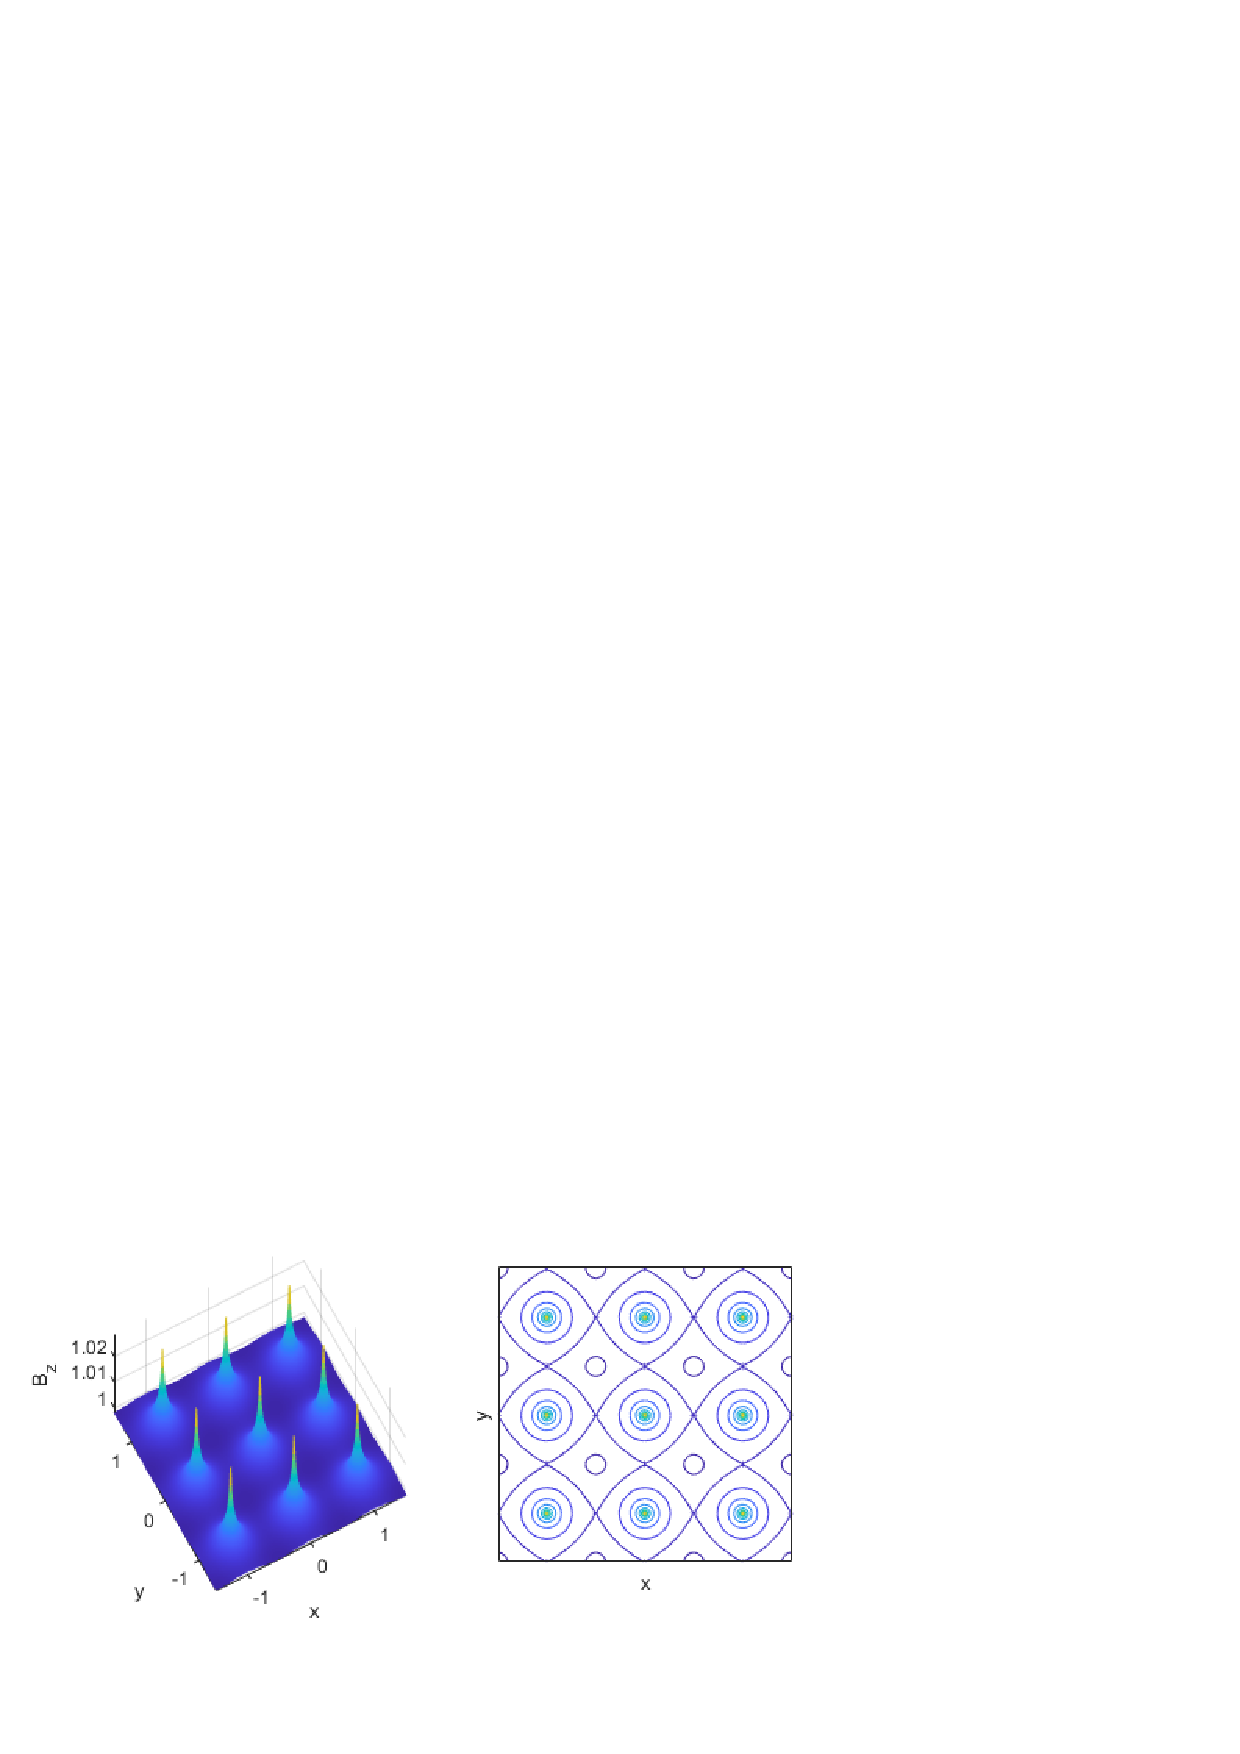
\includegraphics[width=\maxwidth{56.196688409433015em}]{figure_0.png}
\end{center}
\begin{center}
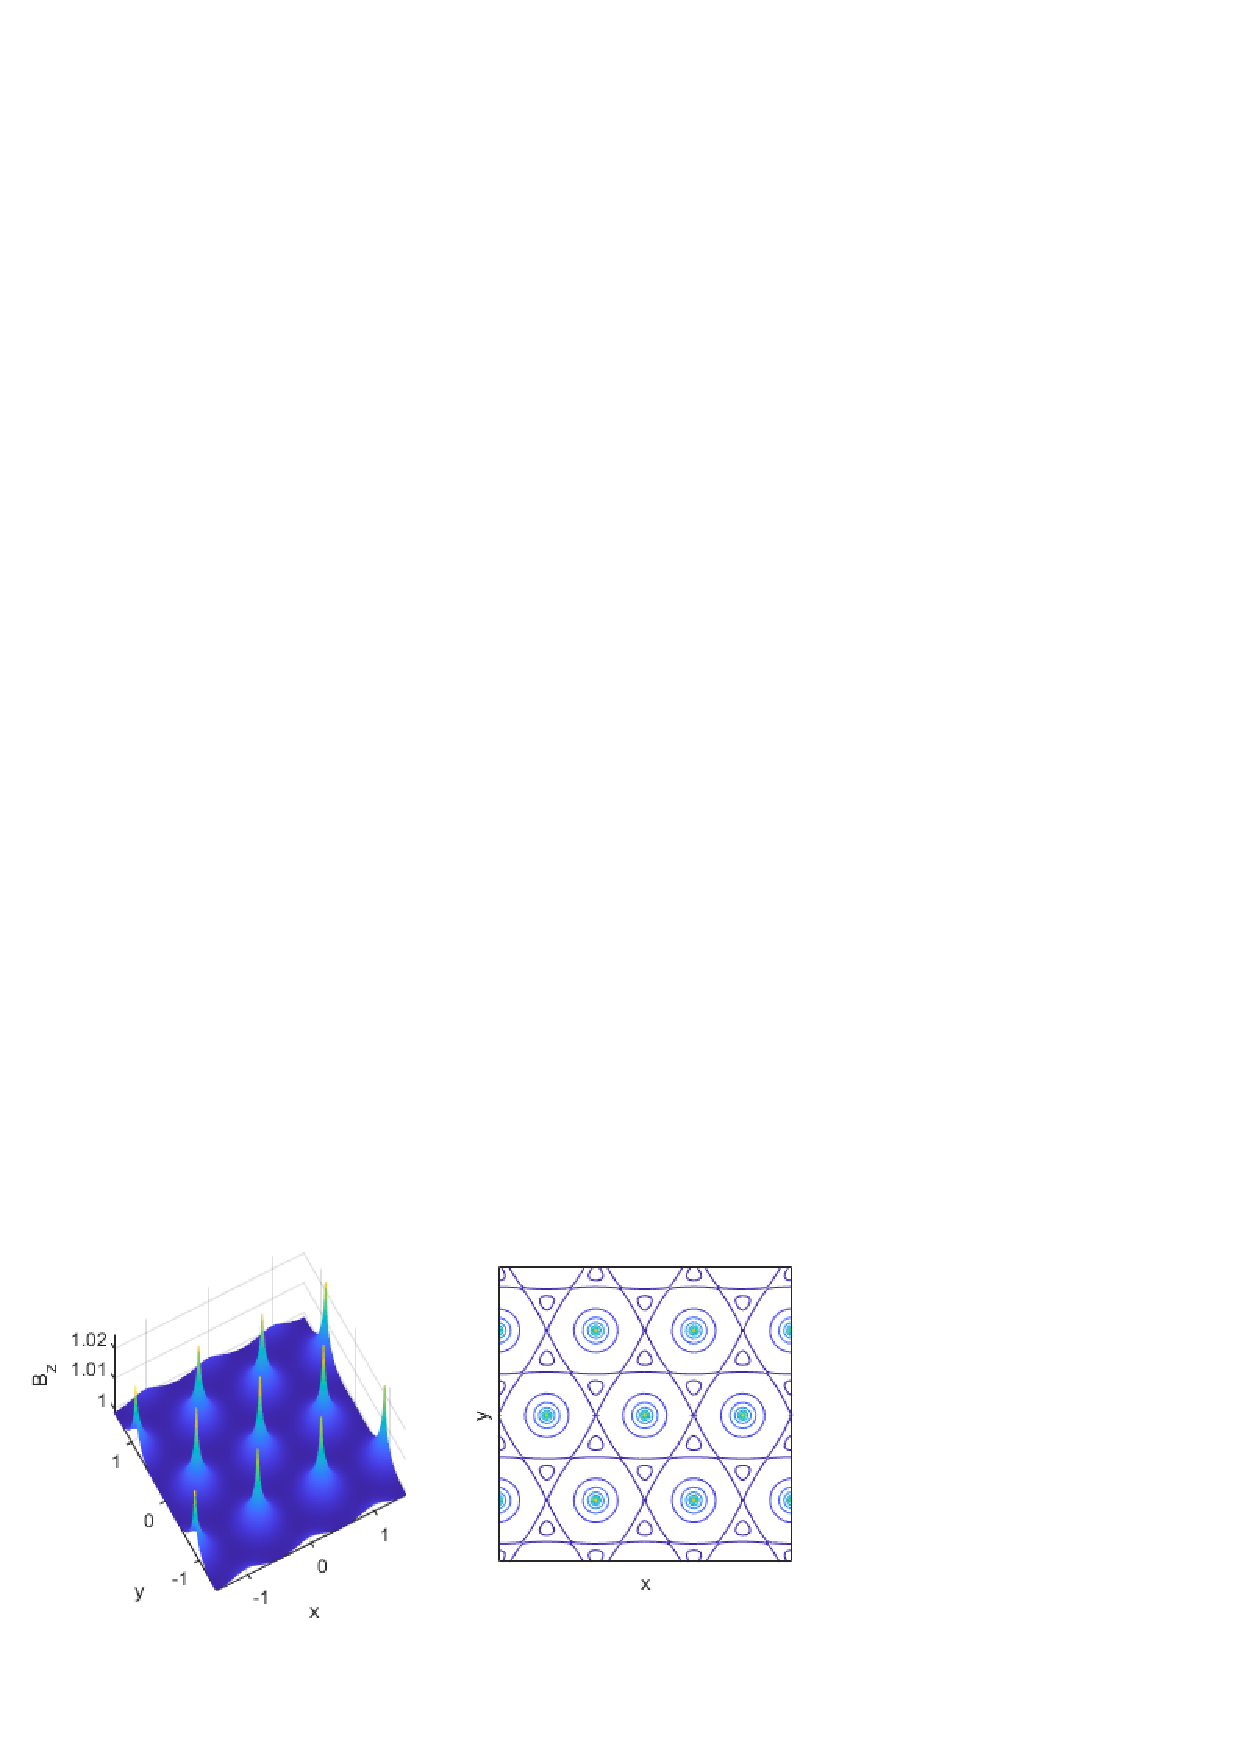
\includegraphics[width=\maxwidth{56.196688409433015em}]{figure_1.png}
\end{center}

\begin{par}
\begin{flushleft}
Flux pinning due to impurity:
\end{flushleft}
\end{par}

\begin{matlabcode}
run('fluxPinPlot.m')
\end{matlabcode}
\begin{matlaboutput}
Warning: Vectorized content might take a long time to create, or it might contain unexpected results. Set 'ContentType' to 'image' for better performance. Click here to not see this message again.
\end{matlaboutput}
\begin{center}
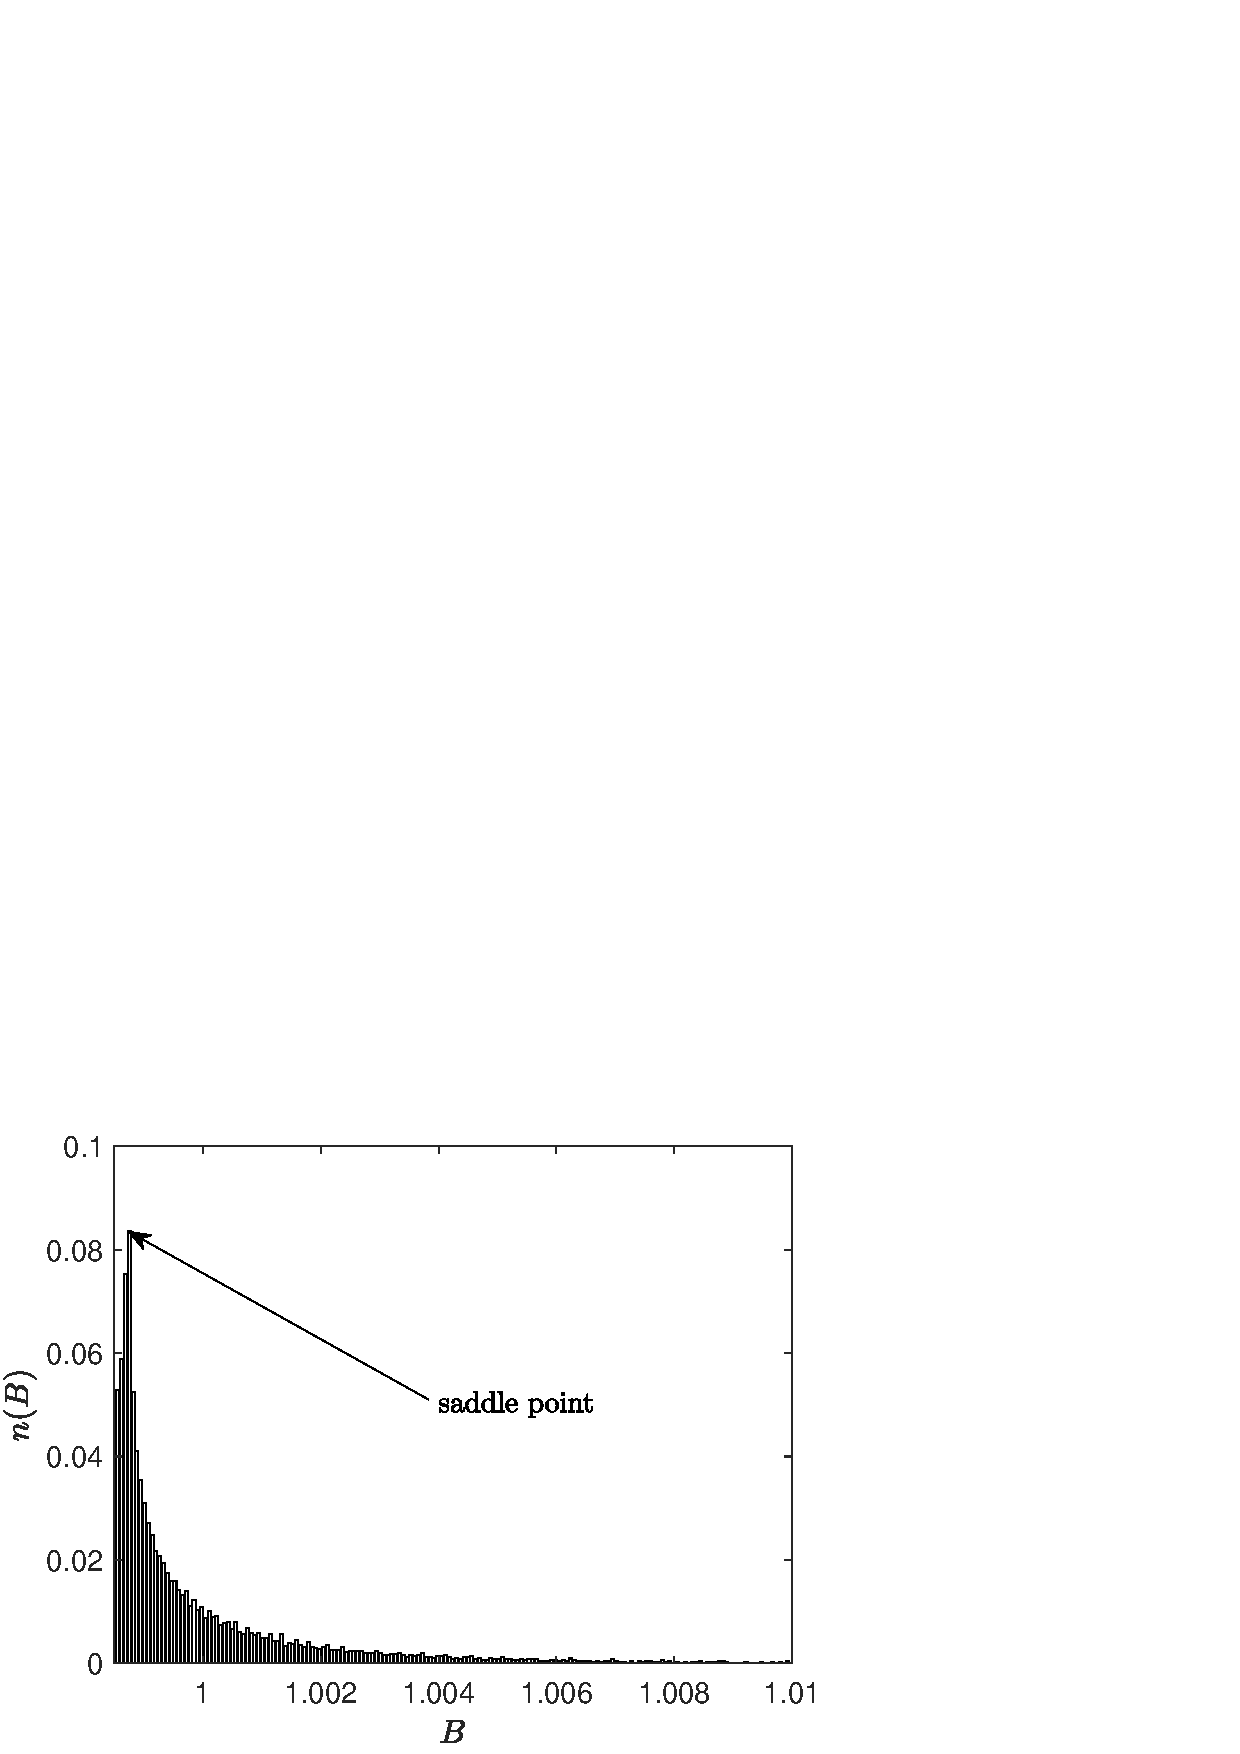
\includegraphics[width=\maxwidth{56.196688409433015em}]{figure_2.png}
\end{center}

\matlabheading{Supercurrent}

\begin{par}
\begin{flushleft}
The superconducting order parameter can be calculated with\texttt{ }\href{./supercurrent.m}{\texttt{supercurrent(in, eigenE, eigenV)}}.
\end{flushleft}
\end{par}

\begin{par}
\begin{flushleft}
\texttt{in - Struct defining the BCS Hamiltonian}
\end{flushleft}
\end{par}

\begin{par}
\begin{flushleft}
\texttt{eigenV - Unitary transformation matrix of BCS Hamiltonian}
\end{flushleft}
\end{par}

\begin{par}
\begin{flushleft}
\texttt{eigenE - Diagonalized matrix of BCS Hamiltonian }
\end{flushleft}
\end{par}


\vspace{1em}
\begin{par}
\begin{flushleft}
\href{./supercurrentCompute.m}{\texttt{supercurrentCompute.m}}\texttt{ }can be used to collect the necessary data, i.e. variable after finding self-consistent SCOP and initialization parameters.
\end{flushleft}
\end{par}


\vspace{1em}
\begin{par}
\begin{flushleft}
Supercurrent of SC in magnetic field:
\end{flushleft}
\end{par}

\begin{matlabcode}
run('supercurrentPlot.m')
\end{matlabcode}
\begin{center}
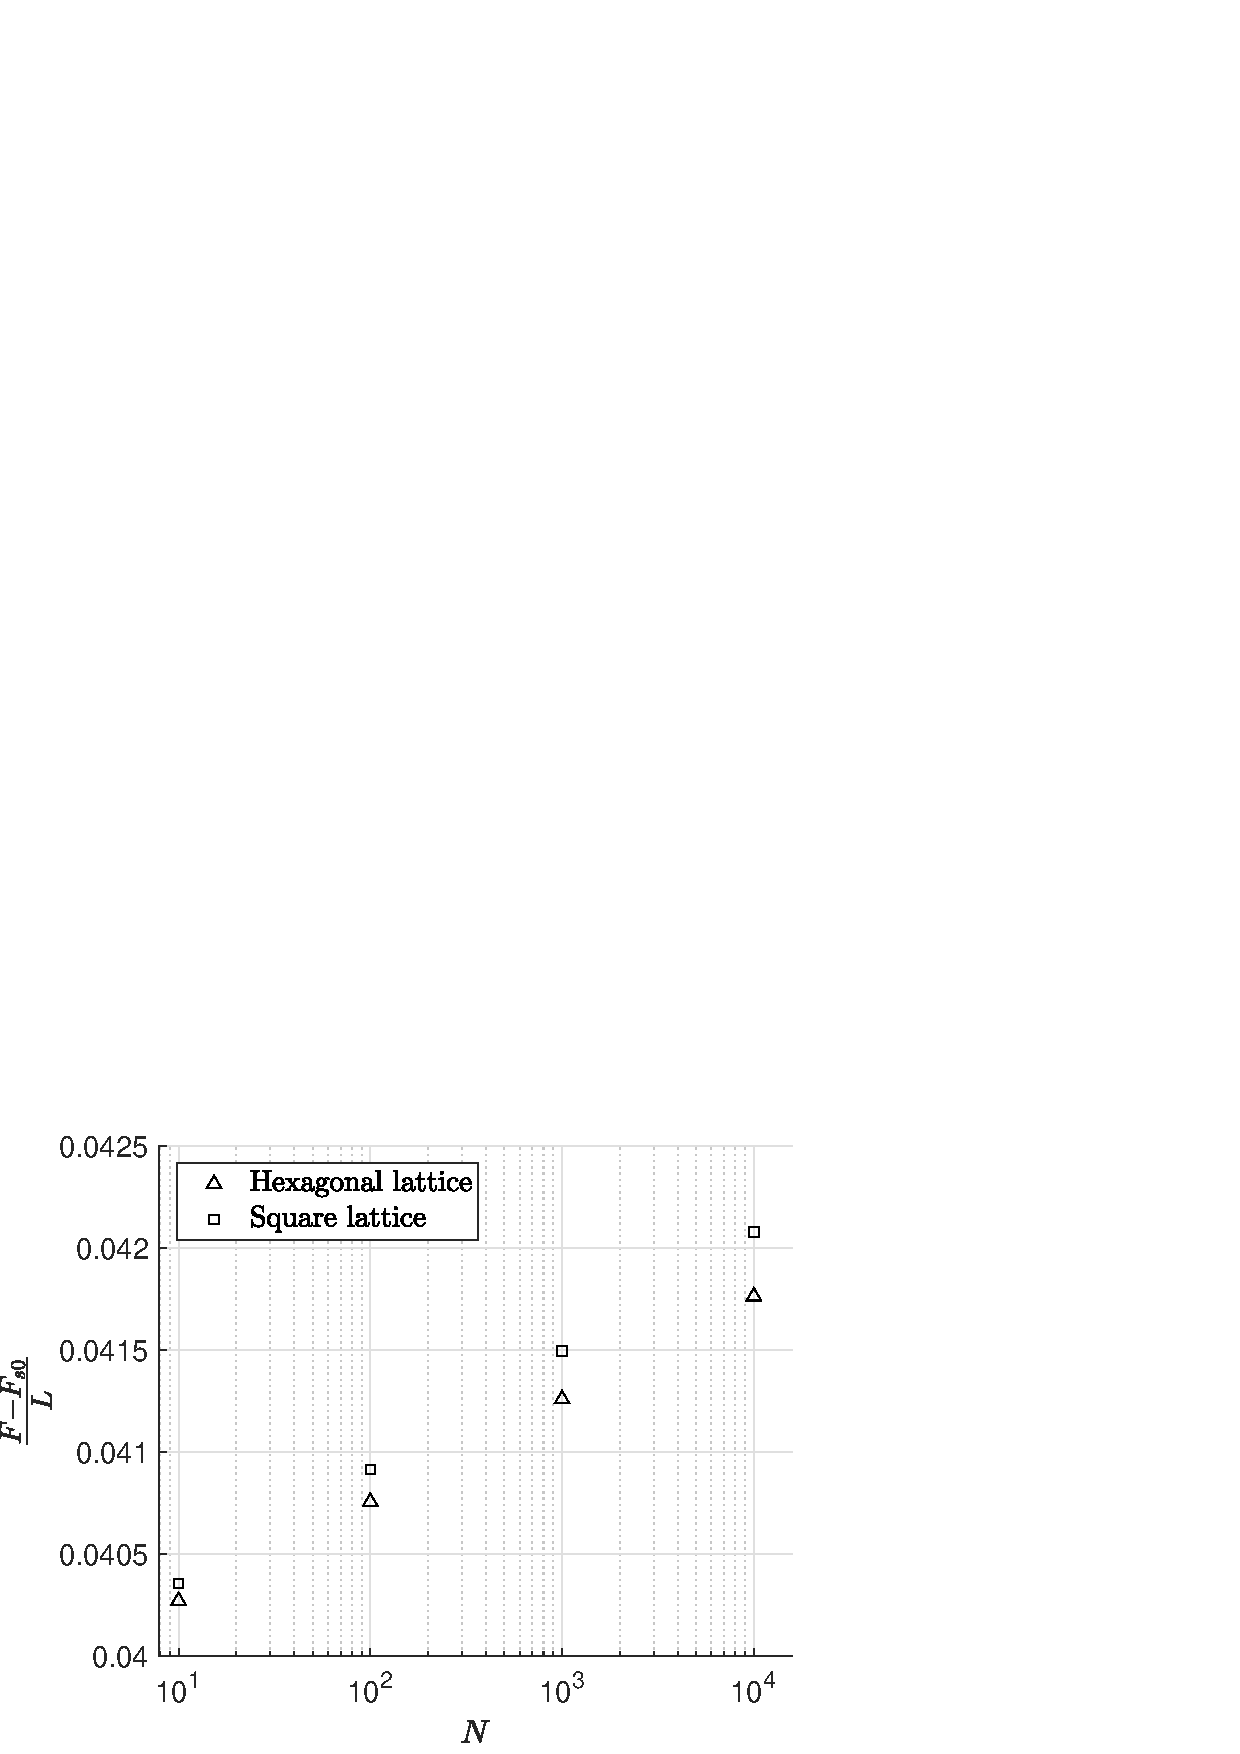
\includegraphics[width=\maxwidth{56.196688409433015em}]{figure_3.png}
\end{center}

\matlabheading{Free Energy}

\begin{par}
\begin{flushleft}
The free energy can be calculated with\texttt{ }\href{./freeEnergyBCS.m}{\texttt{freeEnergyBCS(in, eigenV, eigenE)}}.
\end{flushleft}
\end{par}

\begin{par}
\begin{flushleft}
\texttt{in - Struct defining the BCS Hamiltonian}
\end{flushleft}
\end{par}

\begin{par}
\begin{flushleft}
\texttt{eigenV - Unitary transformation matrix of BCS Hamiltonian}
\end{flushleft}
\end{par}

\begin{par}
\begin{flushleft}
\texttt{eigenE - Diagonalized matrix of BCS Hamiltonian}
\end{flushleft}
\end{par}


\vspace{1em}
\begin{par}
\begin{flushleft}
\href{./freeEnergyCompute.m}{\texttt{freeEnergyCompute.m}}\texttt{ }can be used to calculate free energies of both normal metal and SC, for comparison.
\end{flushleft}
\end{par}


\vspace{1em}
\begin{par}
\begin{flushleft}
Free energy comparison:
\end{flushleft}
\end{par}

\begin{matlabcode}
run('freeEnergyPlot.m')
\end{matlabcode}
\begin{matlaboutput}
Warning: Imaginary parts of complex X and/or Y arguments ignored.
\end{matlaboutput}
\begin{center}
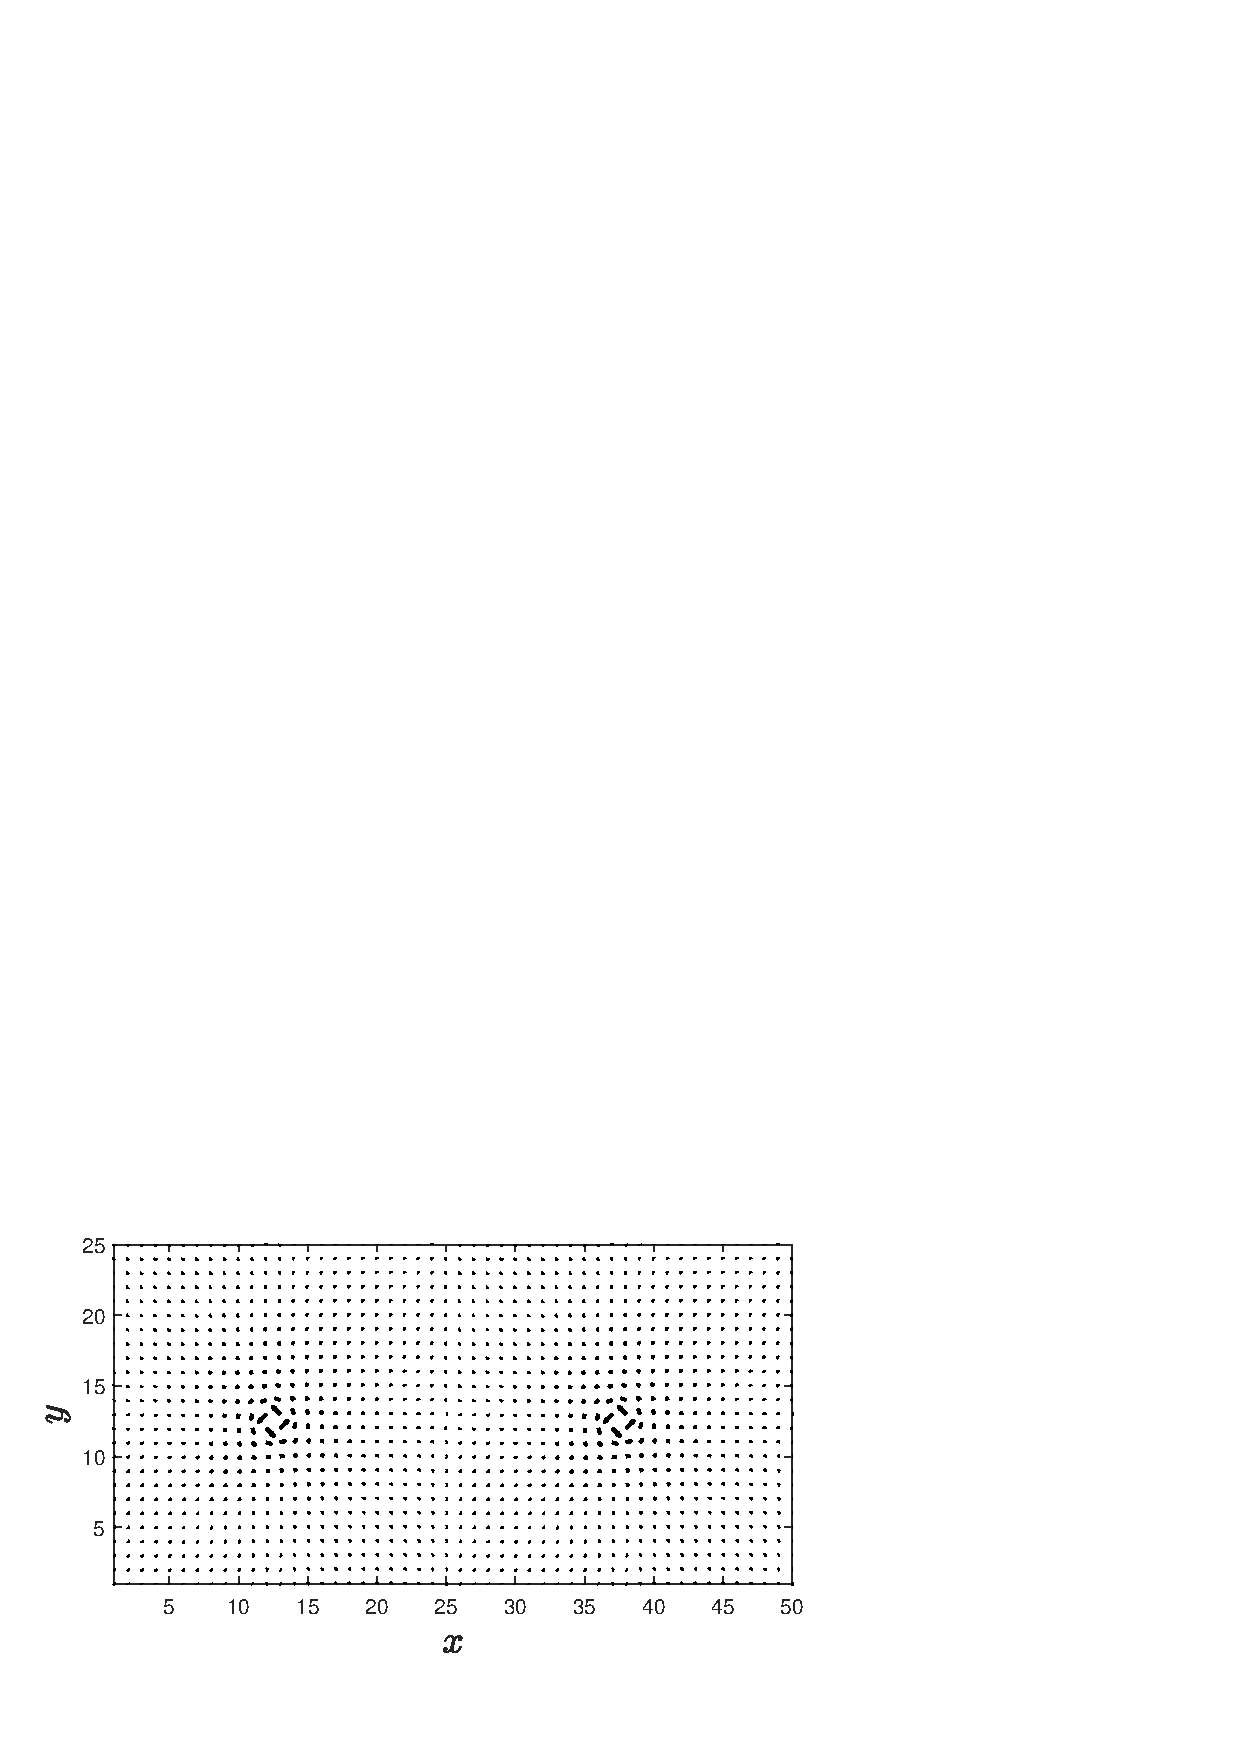
\includegraphics[width=\maxwidth{56.196688409433015em}]{figure_4.png}
\end{center}

\end{document}
